\chapter{Desenvolvimento}

A partir de uma análise sobre qualidade de \textit{software}, métricas de qualidade e fundamentos teóricos do funcionamento do CSS, construiu-se uma pesquisa exploratória, em forma de um questionário, para identificação dos aspectos mais relevantes no processo de manutenção de uma folha de estilo e das características do código fonte que estão relacionadas a sua qualidade.

\section{Construindo o questionário}
Elaborou-se o questionário com os seguintes objetivos:

\begin{itemize}
	\item Identificar os aspectos da linguagem que mais impactam na legibilidade do código;
	\item Identificar os parâmetros que definem qualidade de código no ponto de vista dos entrevistados;
	\item Identificar aspectos mais custosos para manutenção;	
\end{itemize}

A partir da coleta das respostas, pode-se analisar os pesos de cada aspecto de qualidade do código CSS em função de sua manutenibilidade. Identificando as maiores ocorrências de efeitos colaterais, quais são as técnicas para manutenção da legibilidade mais utilizadas e quais são os aspectos de organização do código mais relevantes.

\begin{figure}[!htb]
	\centering
	\caption{Exemplo de questão aplicada no questionário.}
	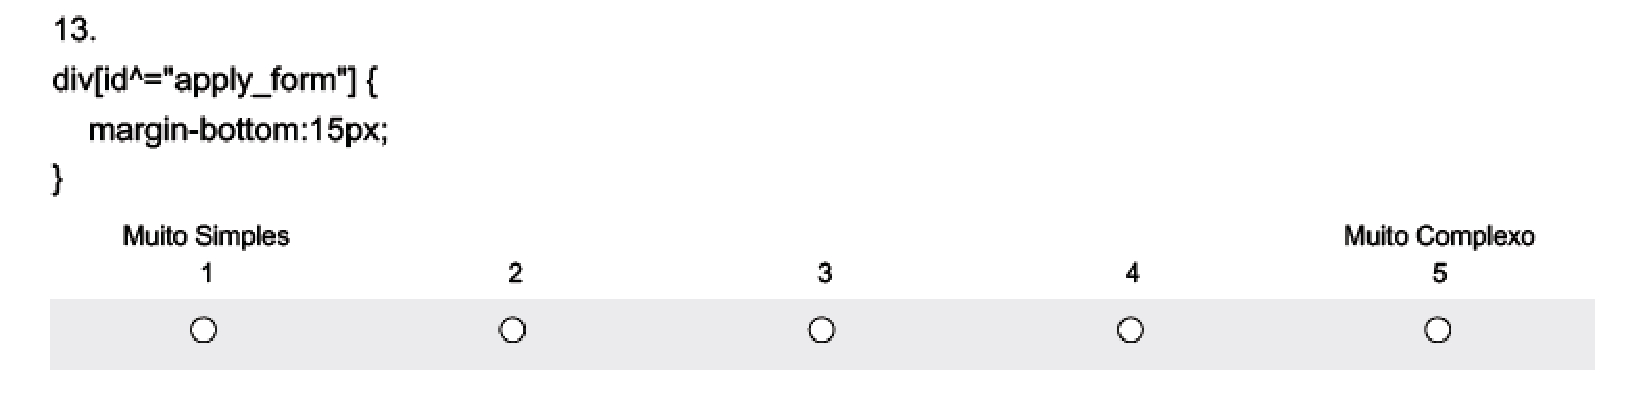
\includegraphics[width=1\textwidth]{./04-figuras/questionario_q13}
	\fonte{Próprio autor}
	\label{fig:questionario_q13}
\end{figure}

Viu-se necessária a avaliação da complexidade de alguns aspectos da linguagem a partir do ponto de vista do profissional, para tal, o questionário (\autoref{chap:apendiceA}) foi construído com uma seção onde é avaliada, com base em um trecho de código (\autoref{fig:questionario_q13}), a dificuldade de se dar manutenção no mesmo. Cada trecho de código foi elaborado de acordo com um aspecto da linguagem que possa causar algum tipo de complicação. Esses aspectos foram escolhidos de acordo com as ponderações e experiência do autor, com base nos estudos realizados.

A dificuldade atribuída por cada pessoa a um determinado conjunto de regras, e propriedades, é subjetiva e depende fortemente da experiência do indivíduo. Portanto construiu-se o questionário com perguntas visando a classificação do respondente de acordo com o seu nível de conhecimento. A partir dessa classificação será possível ponderar as respostas de acordo com o nível de proficiência dos respondentes.

\section{Resultados do Questionário}

O questionário (\autoref{chap:apendiceA}) somou um total de vinte e sete (27) respostas. Este número de respostas pode ser atribuído ao alcance dos meios de divulgação, ou seja, não se fez uso de um canal de comunicação de uso da comunidade de desenvolvedores CSS. Mesmo com um pequeno número de respostas, pôde-se executar uma análise a partir dos resultados da pesquisa. 

Durante os estudos para construção do questionário foram levantas as seguintes hipóteses:

\begin{itemize}
	\item \textbf{(h0)} A manutenção de folhas de estilo não é um trabalho trivial, podendo ocorrer efeitos colaterais durante esta etapa;
	\item \textbf{(h1)} O tamanho da folha de estilo é inversamente proporcional à manutenibilidade;
	\item \textbf{(h2)} Seletores com alta especificidade prejudicam a manutenção da folha de estilo;
	\item \textbf{(h3)} O uso correto de classes, com nomes coerentes, pode ser benéfico para a manutenção;
	\item \textbf{(h4)} A herança de propriedade é um fator causador de efeitos colaterais na etapa de manutenção;
	\item \textbf{(h5)} Seletores de alta complexidade prejudicam na manutenção;
	\item \textbf{(h6)} Regras que não são comumente utilizadas na construção de código CSS podem dificultar a manutenção.
\end{itemize}

O questionário teve então o intuito de validar essas hipóteses, de modo a confirmá-las ou refutá-las. Com uma série de perguntas exploratórias e as específicas, para determinar um valor de escala para os atributos específicos da linguagem.

\subsection{Nível de proficiência}

A primeira questão do questionário (\autoref{chap:apendiceA}) foi desenvolvida com o intuito de classificar os conhecimentos de cada respondente, para assim determinar o seu nível de proficiência. Essa classificação permitiu que os pesos definidos por cada respondente fosse ponderado no resultado final do questionário.

Para esta classificação utilizou-se os critérios apresentados no \autoref{quad:classVsProf}, que indica as funcionalidades do CSS quanto ao seu nível de proficiência.

\begin{quadro}
	\centering
	\caption{Classificação das características do CSS e nível de proficiência}
	\label{my-label}
	\begin{tabular}{|l|l|l|}
		\hline
		\textbf{Iniciante}                                                                         & \textbf{Imtermediário}                                                                                                             & \textbf{Avançado}                                                                        \\ \hline
		\begin{tabular}[c]{@{}l@{}}Localidade\\ Agrupamento\\ Aninhamento\\ Box Model\end{tabular} & \begin{tabular}[c]{@{}l@{}}Herança\\ Transformation\\ Transition\\ Pseudo classes\\ Pseudo elementos\\ Especificidade\end{tabular} & \begin{tabular}[c]{@{}l@{}}At-rules\\ Media queries\\ Animation e keyframes\end{tabular} \\ \hline
	\end{tabular}
	\fonte{Próprio autor}
\end{quadro}


Cada critério recebeu um peso de acordo com sua categoria, sendo 1, 2 e 3 os valores para iniciante, intermediário e avançado, respectivamente. Um respondente foi considerado iniciante se somasse 12 ou menos em suas respostas, intermediário para o respondente que somasse de 13 a 20, e avançado caso suas respostas somassem 21 ou mais. 
%Dessa forma não seria necessário que o respondente tivesse conhecimento sobre todas as regras para ser considerado avançado e também impede que o seja somente por conhecer as regras avançadas. 

\subsection{Visão Geral}

As respostas para o questionário formaram um conjunto de dados capaz de validar as hipóteses levantadas, não de forma definitiva, mas com dados suficientes para construção da métrica.

As questões propostas para identificar os aspectos de qualidade do código CSS identificaram resultados diversos. Como na \autoref{fig:questionario_q2}, podemos verificar que mais de 90\% dos respondentes identificaram os elementos estruturais, a nomenclatura coerente para as classes e identificadores (\texttt{id}) como sendo imprescindíveis para qualidade da folha de estilo.

\begin{figure}[!htb]
	\centering
	\caption{Resultado da questão 2 do questionário \autoref{chap:apendiceA}.}
	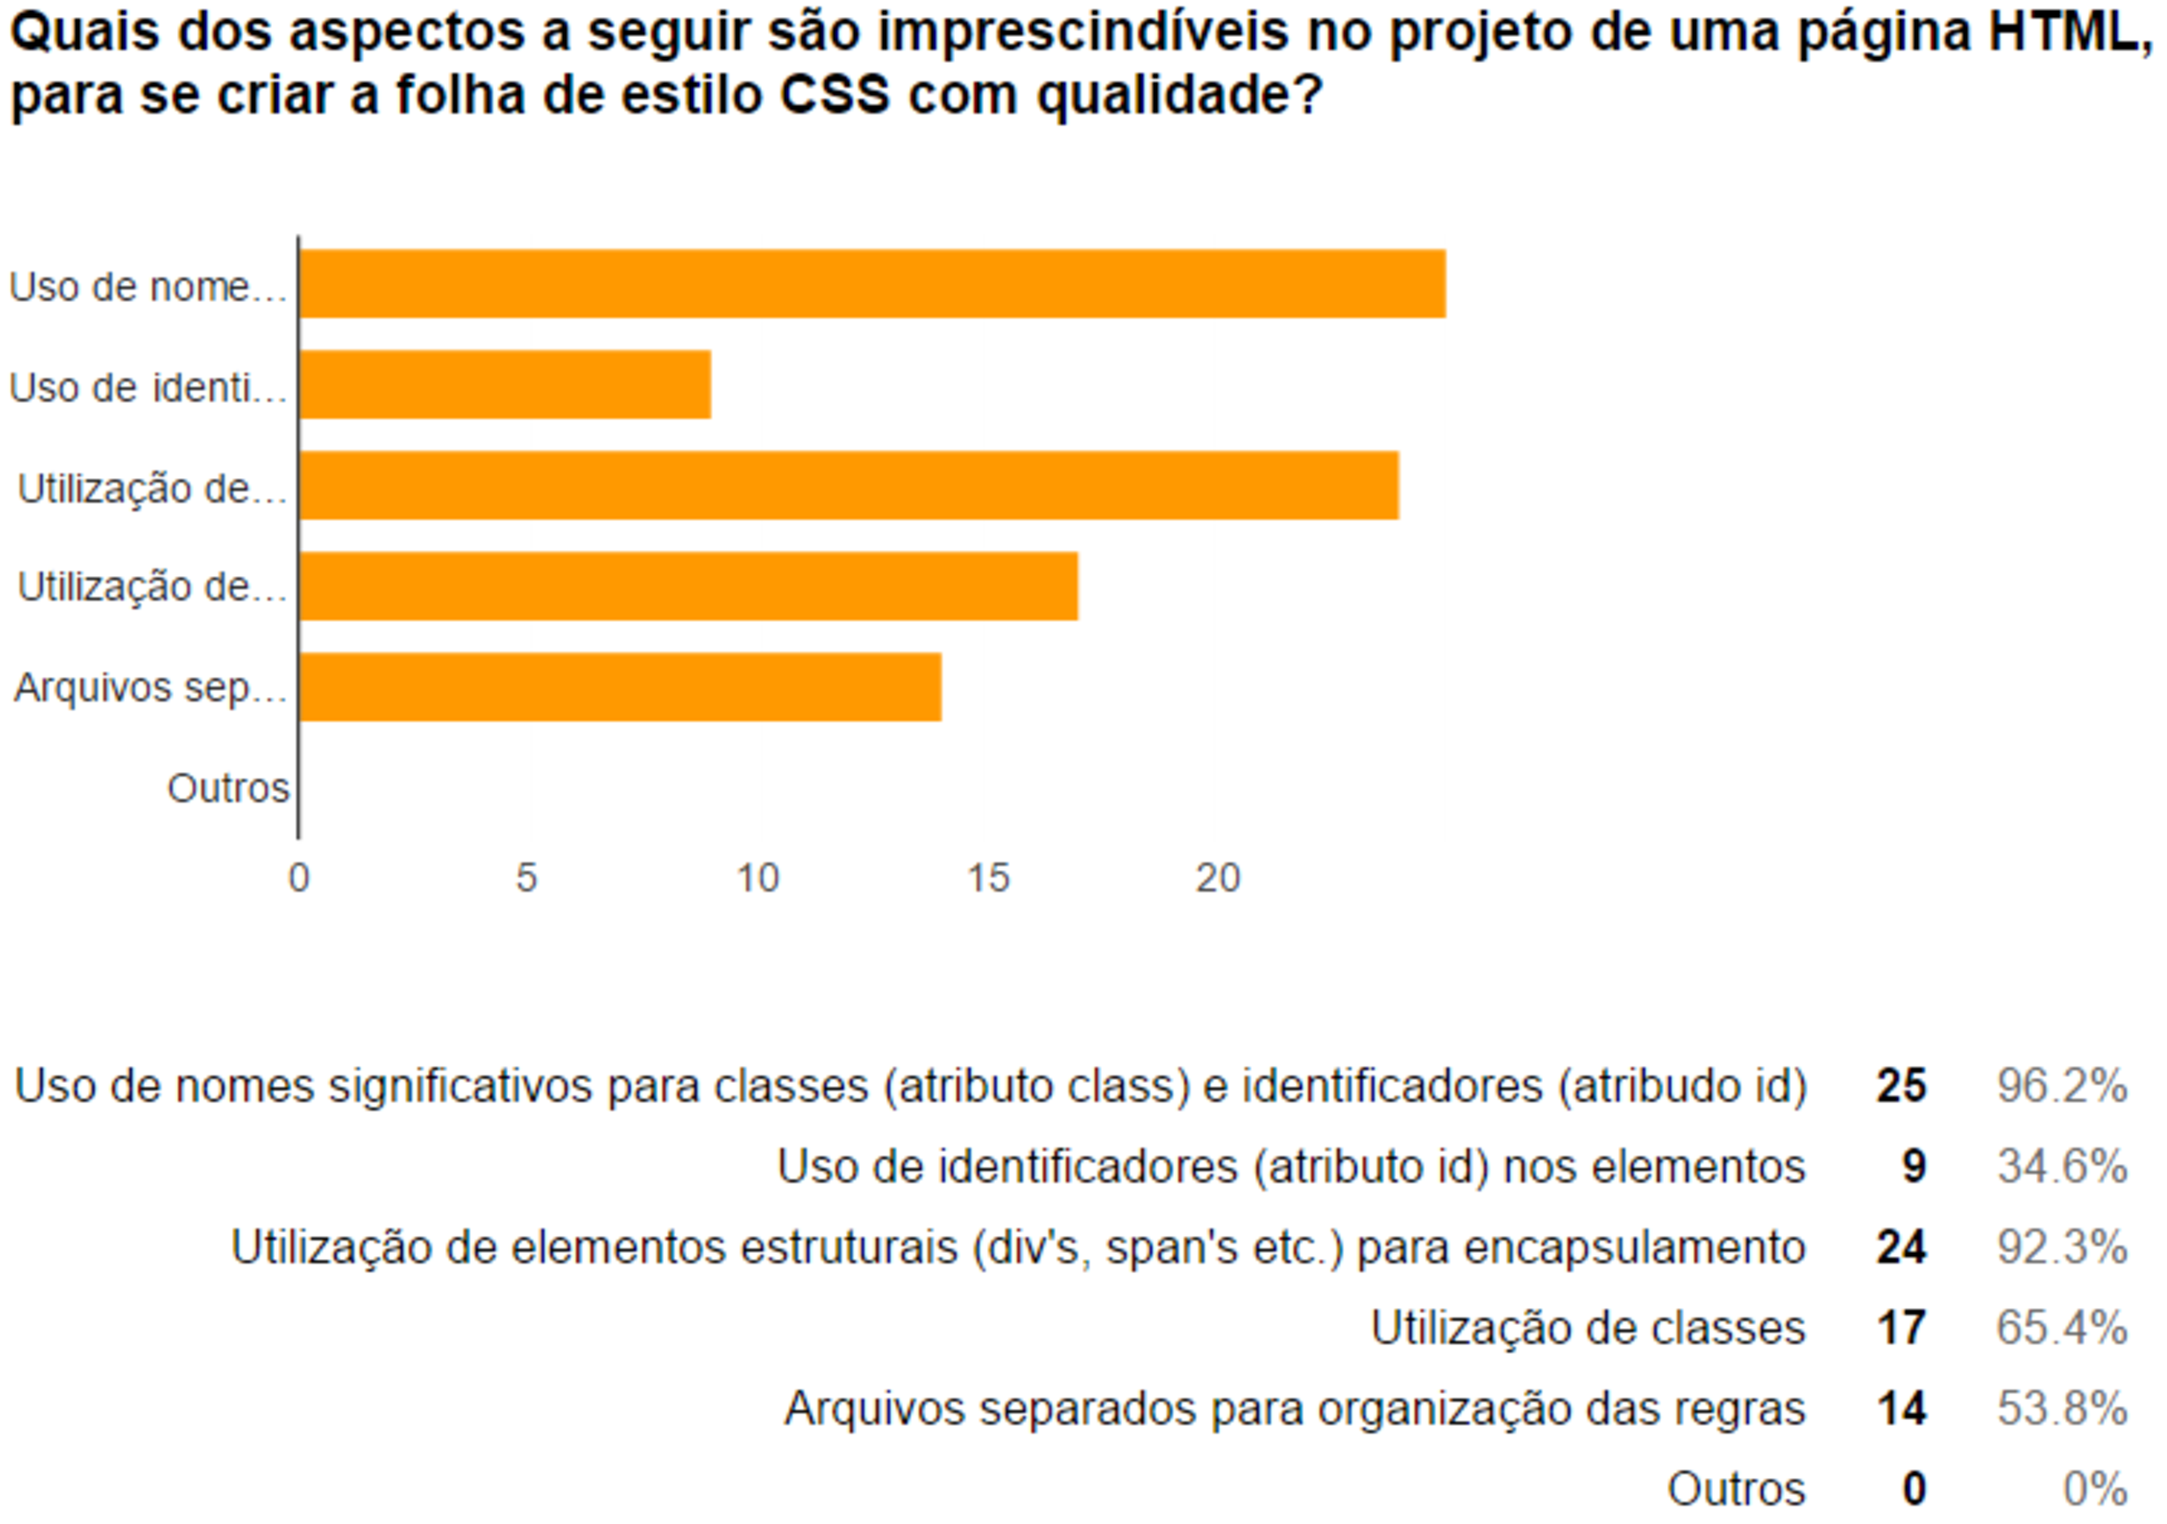
\includegraphics[width=1\textwidth]{./04-figuras/questionario_q2}
	\fonte{Próprio autor}
	\label{fig:questionario_q2}
\end{figure}

Estas respostas corroboram com a hipótese h3, mostrando que a boa estruturação dos elementos do documento de conteúdo, impactam diretamente na construção da folha de estilo.

Na questão exposta na \autoref{fig:questionario_q3} podemos notar os aspectos do CSS que interferem na qualidade do código. Nota-se aqui que não houve unanimidade para esta questão, porém percebe-se uma maior pontuação nas questões que têm impacto na legibilidade do código, \textit{e.g.} organização em seções e modularidade do código.

\begin{figure}[!htb]
	\centering
	\caption{Resultado da questão 3 do questionário \autoref{chap:apendiceA}.}
	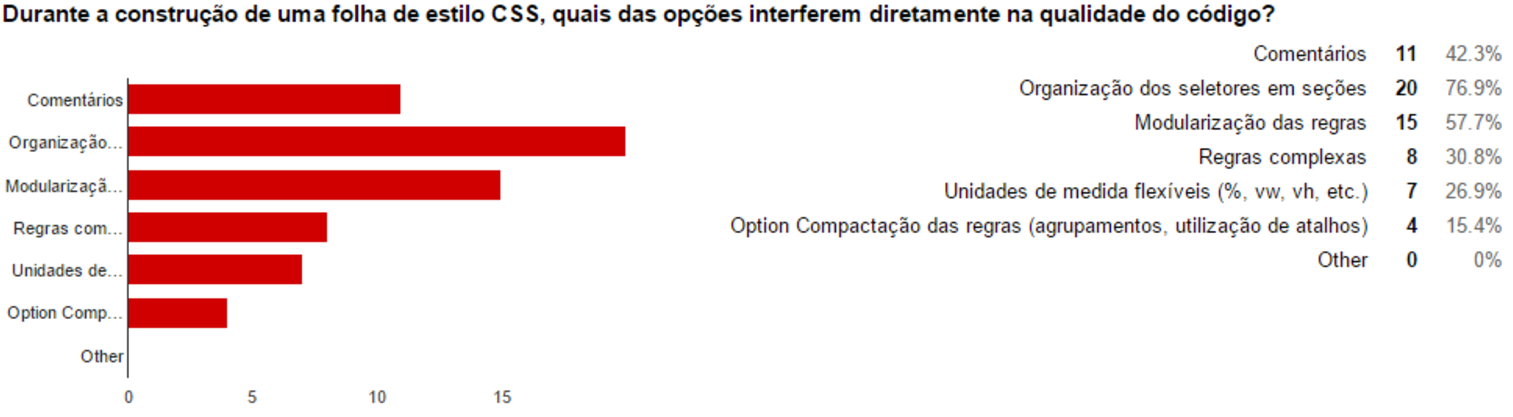
\includegraphics[width=1\textwidth]{./04-figuras/questionario_q3}
	\fonte{Próprio autor}
	\label{fig:questionario_q3}
\end{figure}

Na \autoref{fig:questionario_q9}, é possível verificar que o maior número de ocorrências de efeitos colaterais, para os respondentes, está na fase de manutenção do código. Esse resultado corrobora com a hipótese (h0).

\begin{figure}[!htb]
	\centering
	\caption{Resultado da questão 9 do questionário \autoref{chap:apendiceA}.}
	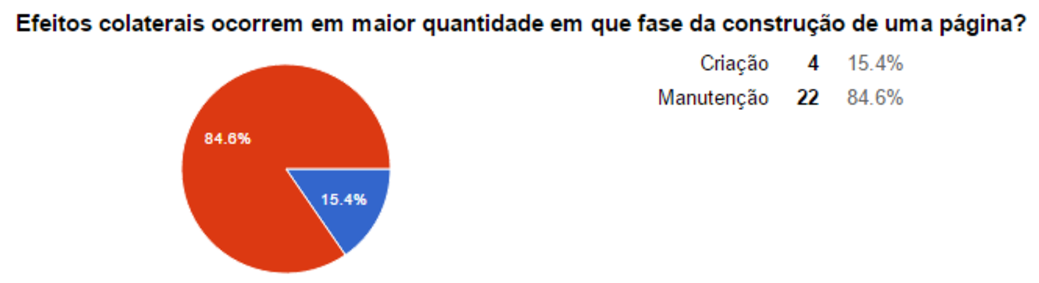
\includegraphics[width=1\textwidth]{./04-figuras/questionario_q9}
	\fonte{Próprio autor}
	\label{fig:questionario_q9}
\end{figure}

Ainda sobre os efeitos colaterais, foi elaborada uma questão com objetivo de identificar quais são as propriedades do CSS que mais os causam. As respostas foram variadas e por isso não foi possível identificar um padrão a partir desta pesquisa. No entanto, as respostas com elementos semelhantes sempre tinham relação com definição de posicionamento e tamanho dos elementos (e.g.: \texttt{position}, \texttt{margin}, \texttt{padding}, \texttt{display}, \texttt{width}, \texttt{z-index}, \texttt{float}, etc). A partir das respostas obtidas pode-se identificar os valores de manutenibilidade para os elementos que possuírem características de herança, prioridade e atuação semelhantes.

\subsection{Questões Exploratórias}

Algumas questões desse questionário tinham o objetivo de captar informações da experiência dos respondentes, a fim de identificar parâmetros que não foram cobertos pelo questionário. Algumas respostas agregaram valor à pesquisa, identificando esses pontos e mostrando algumas informações valiosas acerca da qualidade da folha de estilo. 

Foi questionado quais são os pontos críticos que podem dificultar a manutenção, ou evolução, do código CSS. Das respostas obtidas, pode-se notar no \autoref{qd:openAnswers} aquelas que corroboram ou refutam as hipóteses levantadas.

\begin{quadro}[!htb]
	\centering
	\caption{Contribuição das respostas da questão 6 do questionário. (\autoref{chap:apendiceA})}
	\label{qd:openAnswers}
	\begin{tabular}{|l|c|c|}
		\hline
		\textbf{Resposta}                                                                                                                                                                                                                                                                                                                                                                                                                                                                                                            & \multicolumn{1}{l|}{\textbf{Corrobora}} & \multicolumn{1}{l|}{\textbf{Refuta}} \\ \hline
		Estilizar elementos sem classe, criar folhas de estilos muito extensas.                                                                                                                                                                                                                                                                                                                                                                                                                                                      & h1                                      &                                      \\ \hline
		CSS's que são atribuídos de forma mais genérica aos elementos.                                                                                                                                                                                                                                                                                                                                                                                                                                                                &                                         & h2                                   \\ \hline
		\begin{tabular}[c]{@{}l@{}}Regras complexas \\ Herança de valor de propriedade (valores,inherit, initial)\\ Aninhamento (seleção de elementos aninhados)\end{tabular}                                                                                                                                                                                                                                                                                                                                                  & h5                                      &                                      \\ \hline
		\begin{tabular}[c]{@{}l@{}}Utilização de nomes muitos genéricos para classes ou atributos.\\ A estilização que não é mais usada e fica no código.\end{tabular}                                                                                                                                                                                                                                                                                                                                                               & h3;h6                                   &                                      \\ \hline
		\begin{tabular}[c]{@{}l@{}}Regras para itens muito genéricos. \\ Utilização de !imporant. \\ Código repetido.\end{tabular}                                                                                                                                                                                                                                                                                                                                                                                                   & h6                                      & h2                                   \\ \hline
		Saber se um seletor está ou não sendo usado em algum parte do código.                                                                                                                                                                                                                                                                                                                                                                                                                                                        & h6                                      &                                      \\ \hline
		Seletores muito específicos.                                                                                                                                                                                                                                                                                                                                                                                                                                                                                                  & h2                                      &                                      \\ \hline
		\begin{tabular}[c]{@{}l@{}}Regras com seletores muito gerais, como classes e tags, \\ costumam provocar efeitos colaterais com mais frequência.\\ Acho que para poder escrever regras desse tipo (gerais), \\ todas as propriedades sendo definidas precisam ser "óbvias" \\ (fácil de uma 3ª pessoa entender por que ela está ali) \\ e também gerais (não sendo algo como uma classe .button \\ definindo um left:54px, que deveria estar sendo aplicado \\ a apenas um .button em particular e não a todos).\end{tabular} & h2                                      &                                      \\ \hline
		\begin{tabular}[c]{@{}l@{}}Arquivo desorganizado, regras repetidas, \\ sem sessões definidas,código compactado.\end{tabular}                                                                                                                                                                                                                                                                                                                                                                                                  & h3;h6                                   &                                      \\ \hline
	\end{tabular}
	\fonte{Próprio autor, a partir de respostas do questionário}
\end{quadro}

Essas respostas foram de suma importância para identificação de quais os critérios que deveriam, ou não, ser considerados para a avaliação da folha de estilo. Depois de identificados esses critérios, foi feita a análise das questões com exemplos de código, com o objetivo de definir os seus pesos.

\subsection{Cálculo dos pesos}

A última seção de perguntas no questionário foi desenvolvida com a intenção de identificar as dificuldades dos respondentes, quando deparados com uma situação de código CSS. As propriedades e regras exemplificadas foram desenvolvidas com objetivos específicos, cada uma delas cobrindo uma das características que representavam, na visão do autor, um fator dificultador na modificação de uma folha de estilo.

Cada respondente identificou em uma escala (1 a 5) a dificuldade de se dar manutenção no trecho de código apresentado. Fez-se então uma média de cada resposta, para determinarmos a dificuldade de cada uma das 16 questões.
Pode-se notar na \autoref{fig:graph_scaleMean} a diferença de dificuldade encontrada pelos respondentes com diferentes níveis de proficiência.

\begin{figure}[!htb]
	\centering
	\caption{Média de dificuldade por nível de proficiência em cada uma das questões de escala.}
	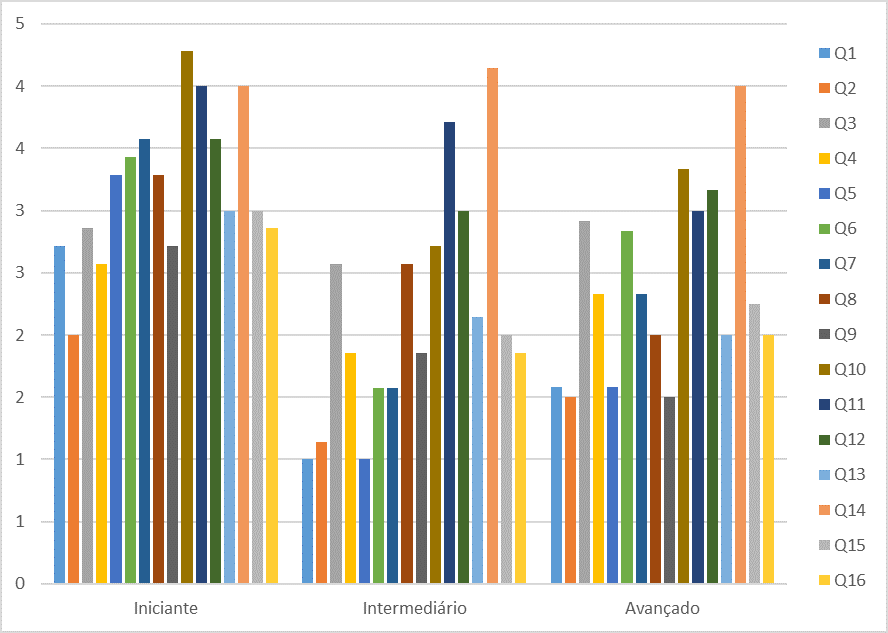
\includegraphics[width=1\textwidth]{./04-figuras/graph_scaleMean}
	\fonte{Próprio autor}
	\label{fig:graph_scaleMean}
\end{figure}

É possível notar a proximidade das respostas dos níveis intermediário e avançado, mas ainda assim as médias do nível avançado são ligeiramente maiores que as do nível intermediário. Os pesos de cada critério foi identificado a partir da média ponderada de cada questão, para evitar que o peso de cada resposta fosse completamente dependente das respostas dos respondentes identificados como iniciantes.

\section{Criação da métrica}
	
A partir das hipóteses levantadas e dos resultados obtidos no questionário, foram identificados pesos para os critérios de avaliação, como visto na \autoref{tab:tabelaPesos}. Esses pesos são utilizados para o cálculo de cada métrica de forma individual, aplicando uma forma de avaliação correspondente a cada um dos critérios.


\begin{table}[!htb]
	\centering
	\caption{Tabela com peso de cada critério avaliado.}
	\label{tab:tabelaPesos}
	\begin{tabular}{l|l}
		\textbf{Critério}                                                           & \textbf{Peso} \\ \hline
		Seletores raros: \{{[}\textasciicircum ={]}, {[}\$={]}, \char`~, +,\textgreater\} & 3             \\
		Agrupamentos                                                                & 2,8           \\
		Aninhamento                                                                 & 2,8           \\
		Propriedade simplificada                                                    & 3,2           \\
		Pseudo elementos                                                            & 2,8           \\
		Seletor com mais de 35 caracteres                                           & 3             \\
		At-rules                                                                    & 2,8           \\
		Media queries                                                               & 3,8           \\
		Prefixos: \{-webkit, -ms, etc.\}                                            & 4,2           \\
		Clausula :not                                                               & 3,8           \\
		Complexidade do seletor                                                     & 4,8           \\
		Seletor de localidade: \{nth-last-child, first-child, etc.\}                & 2,6          
	\end{tabular}
	\fonte{Próprio autor}
\end{table}

Para o cálculo do critério de comprimento do seletor levou-se em consideração um valor de ativação, \textit{i.e.}, a partir de dado número de caracteres o seletor terá um valor de manutenibilidade. Para este valor de ativação utilizou-se dos dados levantados pela pesquisa feita por \citeonline{McPherson:2014}, em que são expostos alguns dados sobre a utilização do CSS na internet. Nesta pesquisa é apresentada uma distribuição do comprimento do seletor em caracteres, como visto na \autoref{fig:distributionLength}. Esta distribuição mostra que a moda dos comprimentos encontrados pela pesquisa é em torno de vinte (20) caracteres. A decisão tomada para o valor de ativação do critério foi então definida como trinta e cinco (35) caracteres, um valor maior que a moda e que possui uma fatia expressiva na distribuição apresentada.

\begin{figure}[!htb]
	\centering
	\caption{Distribuição de tamanho dos seletores}
	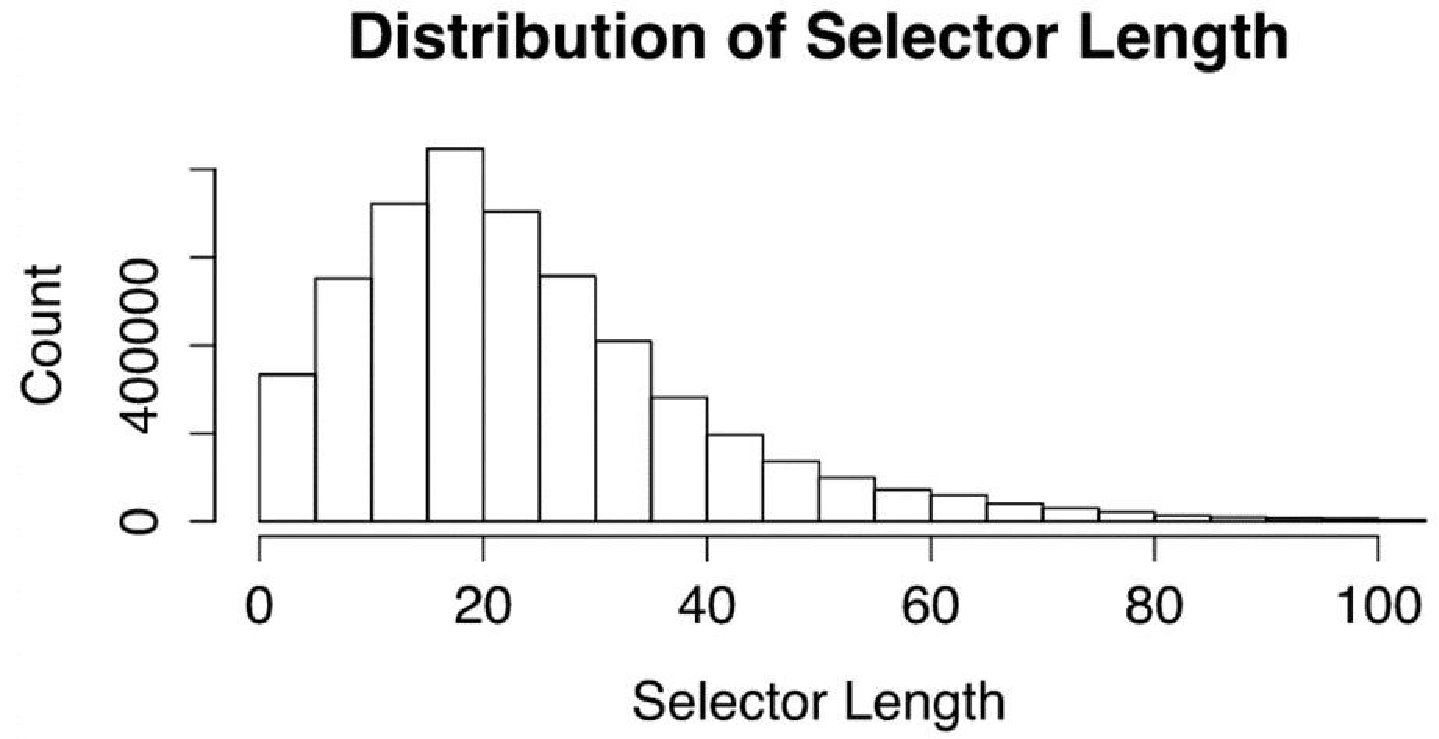
\includegraphics[width=0.8\textwidth]{./04-figuras/dist_selectorL}
	\fonte{\citeonline{McPherson:2014}}
	\label{fig:distributionLength}
\end{figure}

Outros dois critérios de avaliação com cálculos peculiares foram o agrupamento e a complexidade dos seletores. Para o critério de agrupamento foi considerado que a sua manutenibilidade tem um nível de saturação, para esta saturação considerou-se o agrupamento de vinte (20) seletores simples, definido arbitrariamente tomando por base o tamanho modal dos seletores apresentados pela pesquisa de \citeonline{McPherson:2014}. A complexidade deste seletor foi calculada como um crescimento exponencial, onde o peso da dificuldade deste critério é potencializado pela posição do item agregador de complexidade.

Os demais critérios avaliados são calculados pelo número de repetições, faz-se a multiplicação do peso pela quantidade de ocorrências do critério e se obtém o resultado.

Para avaliação da métrica foi criado um \textit{script} que lê a partir do DOM as regras aplicadas sobre o HTML renderizado no navegador. Uma vez que o \textit{script} é executado no navegador, torna-se dependente deste a execução dos testes. Foram necessários alguns testes do \textit{script} para ajustes dos pesos, esses testes foram executados em várias páginas da \textit{web}.

\begin{figure}[!htb]
	\centering
	\caption{Exemplo de resultado da excução do \textit{script} de cálculo da métrica.}
	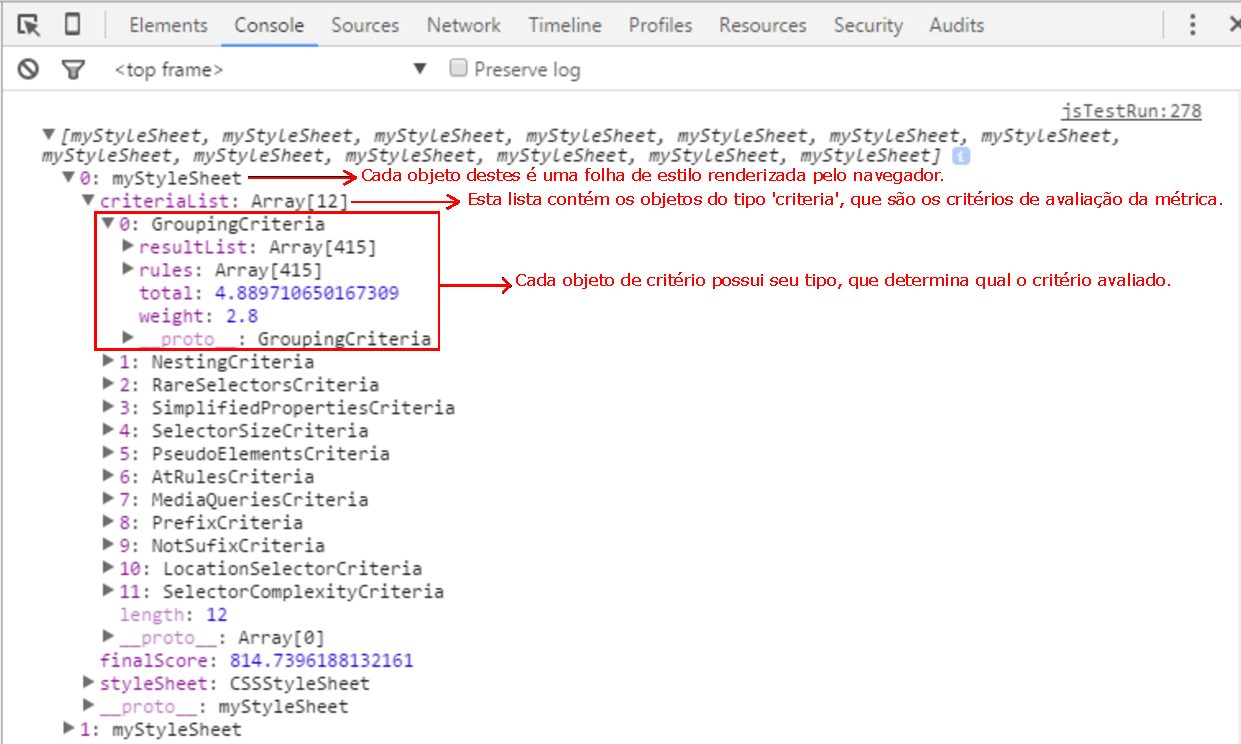
\includegraphics[width=1\textwidth]{./04-figuras/calculator}
	\fonte{Próprio autor}
	\label{fig:calculatorTest}
\end{figure}

O \textit{script} executa os cálculos de cada um dos critérios para cada folha de estilo renderizada, iterando sobre as regras CSS da folha de estilo. Desta forma uma mesma regra será avaliada sobre todos os critérios determinados, uma vez que as regras podem se encaixar em mais de um critério. Ao final da execução do \textit{script} será obtido o resultado total de cada critério em cada folha de estilo, o que permite uma análise da contribuição dos critérios para o resultado final da métrica.

Na \autoref{fig:calculatorTest} pode-se visualizar a estrutura do resultado de uma execução do \textit{script}. O código fonte desse \textit{script} está disponível no repositório GitHub\footnotemark. O objetivo final deste código é gerar um \textit{bookmarklet} que exiba as informações de qualidade do código CSS presente na página \textit{web}.

\footnotetext{Disponível em \url{https://github.com/vcsalvador/jsTestRun}.}

Com o \textit{script} para cálculo da métrica pronto e ajustado, fez-se a escolha de roteiro de testes. Para determinar qual seria a melhor forma de avaliar os resultados do \textit{script} foi necessário escolher projetos em que o estilo da página fosse codificado em arquivos CSS, eliminando a possibilidade de aplicar os testes em projetos que utilizem preprocessadores\footnotemark CSS. Além desta limitação, deveria ser possível analisar um outro indicador de manutenibilidade de código, como tempo de evolução, número de defeitos ou algum índice de retrabalho.

\footnotetext{Linguagens de programação intermediárias que geram código CSS, \textit{e.g.} Sass, Less, Stylus, etc.}

\chapter{Avaliação da Métrica}

O Jenkins\footnotemark, uma aplicação de integração contínua de código aberto, foi escolhido por atender a todas as limitações identificadas. O Jenkins é um projeto maduro, largamente utilizado e com uma comunidade de desenvolvimento ativa. Pode-se ver na \autoref{fig:codeFreqGraph} a quantidade de adições e deleções no código por semana. Ele também foi escolhido como objeto de estudo por utilizar somente código CSS para a construção de suas folhas de estilo.

\footnotetext{Disponível em \url{https://jenkins-ci.org/}}

\begin{figure}[!htb]
	\centering
	\caption{Gráfico de frequência de codificação do Jenkins.}
	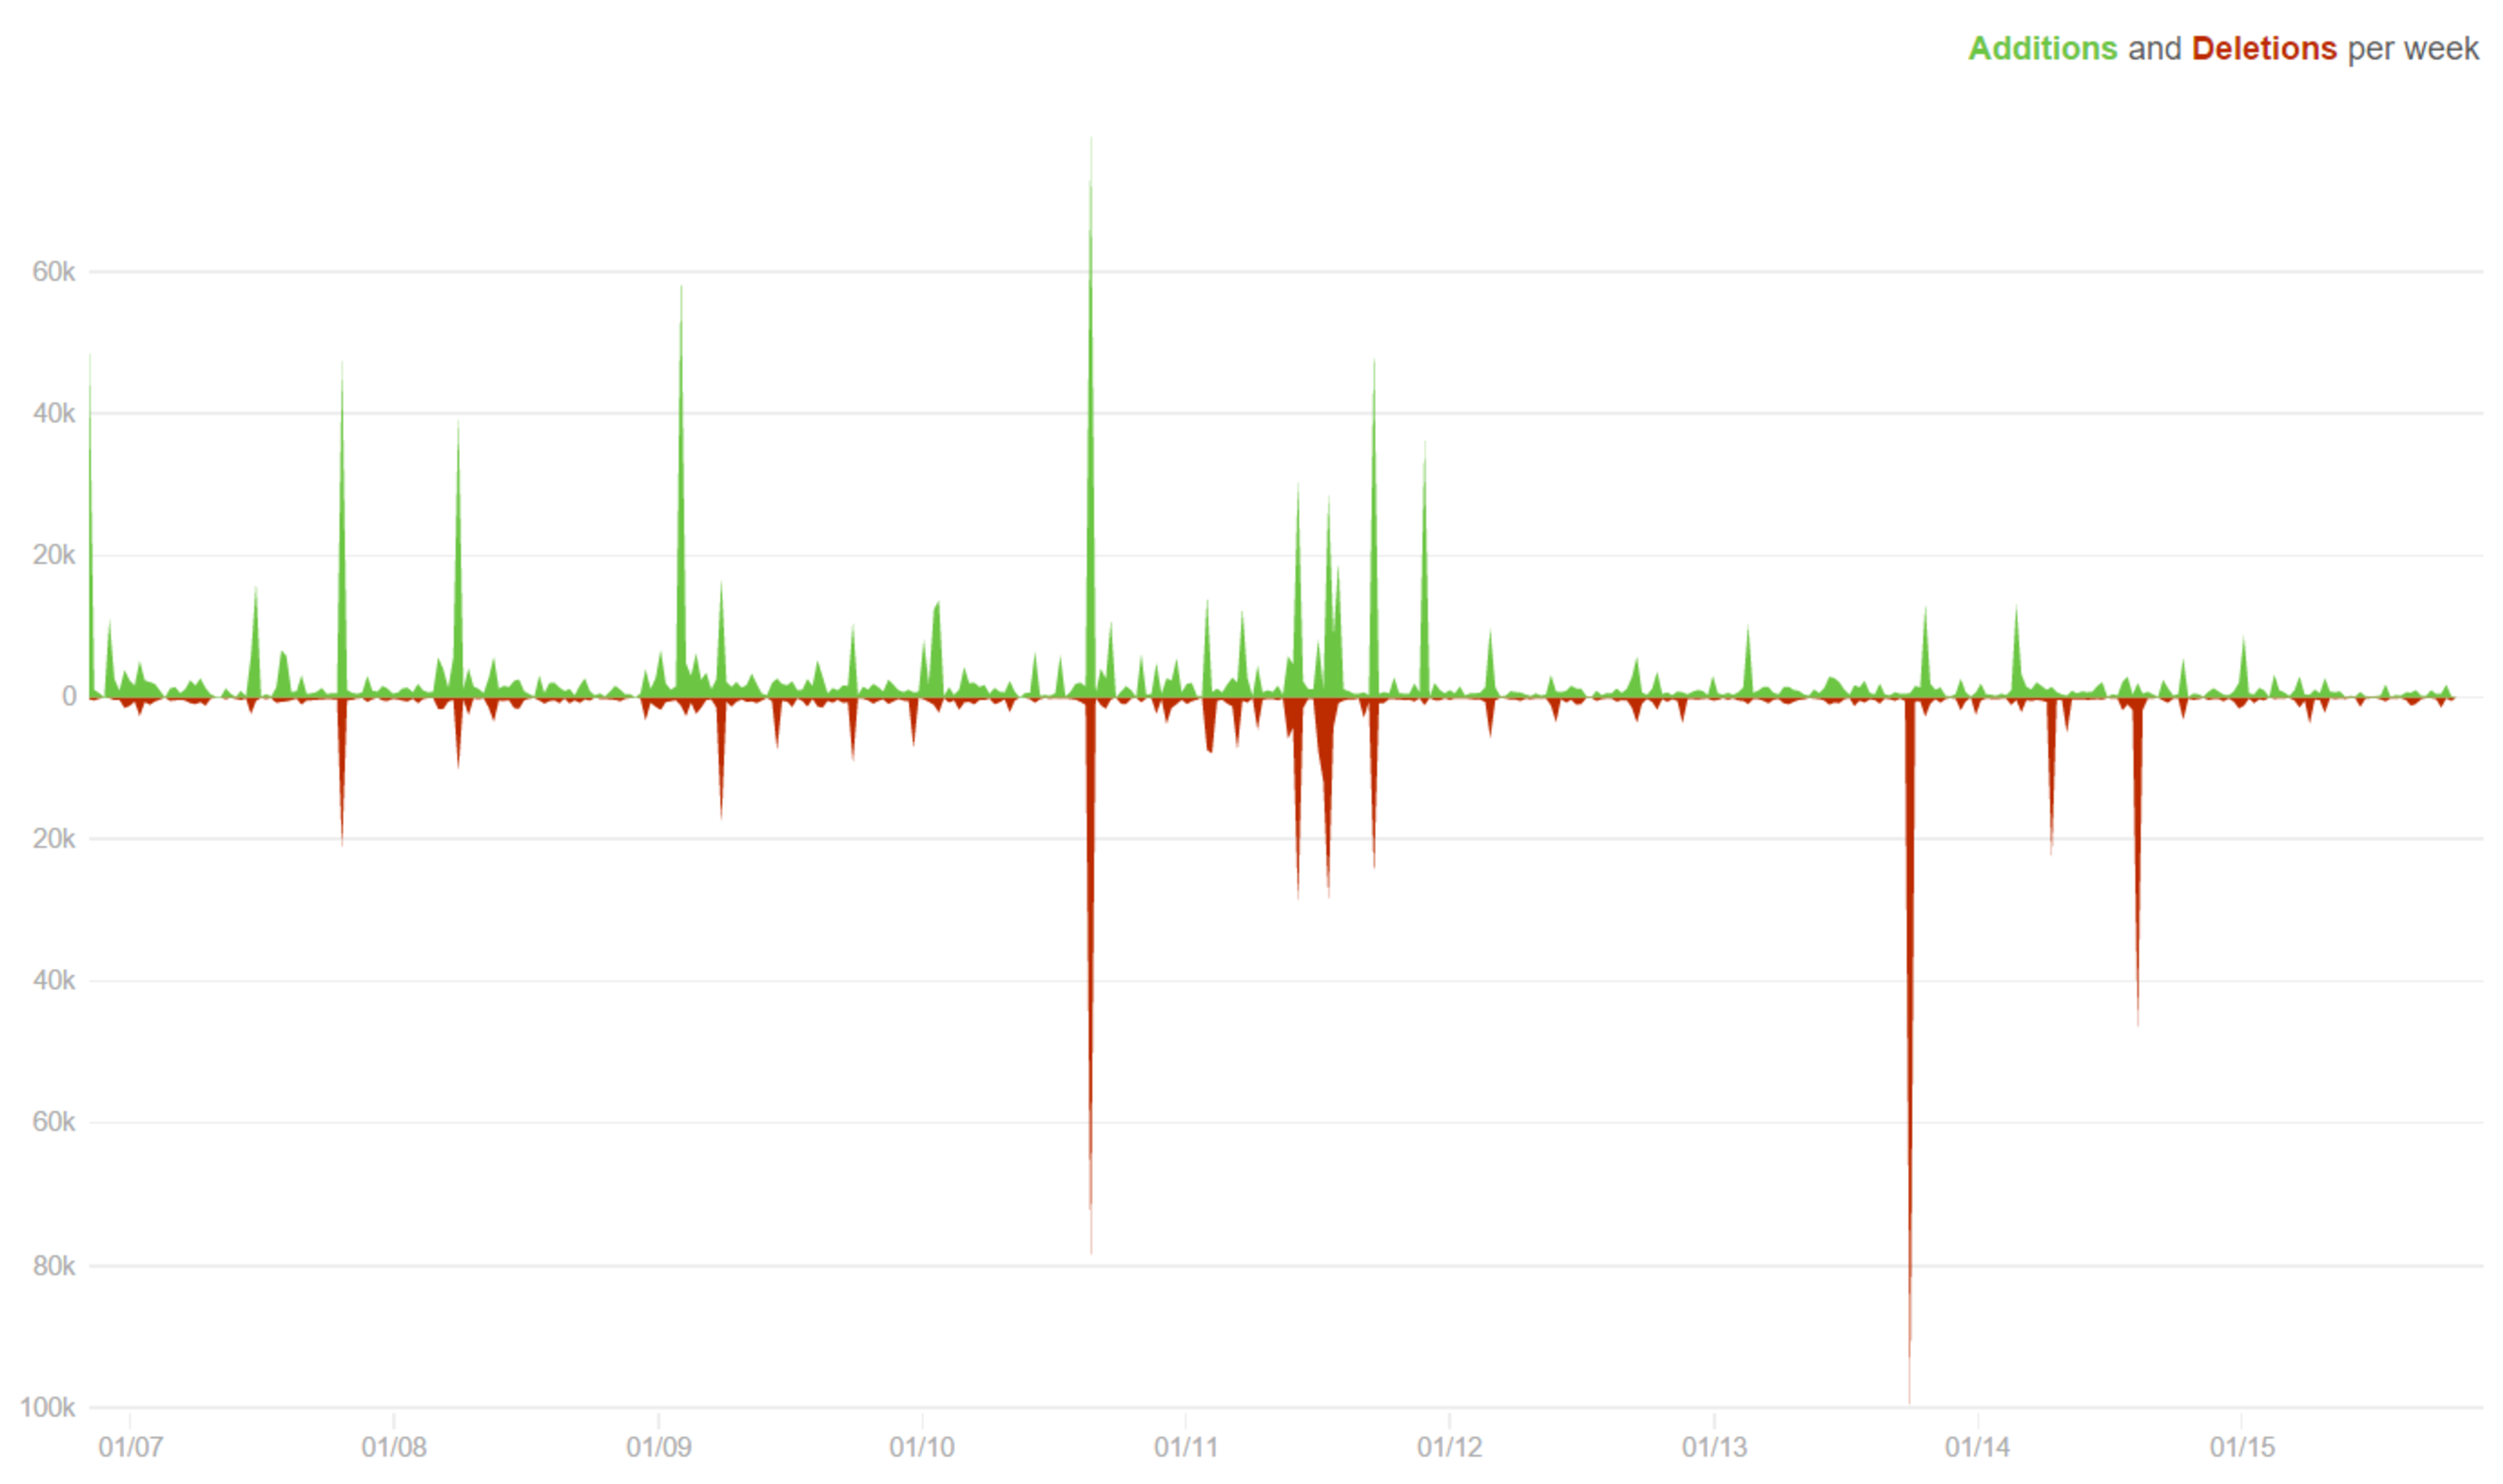
\includegraphics[width=1\textwidth]{./04-figuras/code_freq_graph}
	\fonte{GitHub, disponpível em \url{https://github.com/jenkinsci/jenkins/graphs/code-frequency}. Acessado em 24/10/2015.}
	\label{fig:codeFreqGraph}
\end{figure}

\section{Metodologia de Avaliação}

Para execução dos testes utilizamos doze (12) versões do Jenkins, selecionadas entre as que estão disponibilizadas para download na página do projeto, em intervalos semestrais, para obter dados históricos da aplicação. Essas versões foram escolhidas entre 2010 até a versão mais atual, esta escolha foi feita devido a disponibilidade e possibilidade de identificar em qual ponto no tempo elas foram construídas, conforme exibido no \autoref{tab:versionTabs}.

\begin{quadro}[]
	\centering
	\caption{Versões utilizadas para execução dos testes.}
	\label{tab:versionTabs}
	\begin{tabular}{|l|c|}
		\hline
		\textbf{Versão} & \textbf{Data de lançamento} \\ \hline
		1.369           & 31/07/2010            \\ \hline
		1.395           & 22/01/2011            \\ \hline
		1.423           & 25/07/2011            \\ \hline
		1.450           & 30/01/2012            \\ \hline
		1.475           & 01/08/2012            \\ \hline
		1.500           & 26/01/2013            \\ \hline
		1.525           & 29/07/2013            \\ \hline
		1.549           & 26/01/2014            \\ \hline
		1.574           & 27/07/2014            \\ \hline
		1.598           & 25/01/2015            \\ \hline
		1.622           & 27/07/2015            \\ \hline
		1.633           & 11/10/2015           \\ \hline
	\end{tabular}
	\fonte{Próprio autor}
\end{quadro}

O projeto do Jenkins disponibiliza um meio de se cadastrar e controlar as tarefas relativas ao desenvolvimento da ferramenta (JIRA\footnotemark). Utilizando dos filtros disponíveis no JIRA foi possível identificar as tarefas que tinham alguma relação com os arquivos CSS, tornando possível uma coleta de dados indicadores do período de manutenção do projeto. Devido às características do JIRA, não foi possível a coleta do tempo gasto em cada tarefa, então o indicador escolhido foi a quantidade de defeitos criados a partir da versão de teste.

Com estas informações é possível identificar uma relação entre o valor da métrica e o número de defeitos de cada versão e, a partir disto, determinar o comportamento temporal do código CSS.

\footnotetext{Disponível em \url{https://issues.jenkins-ci.org}}

\section{Dados para Teste}

A partir do repositório\footnote{Disponível em \url{https://updates.jenkins-ci.org/download/war/}} de versões do Jenkins selecionou-se algumas de forma a cobrir uma janela de tempo razoável para as avaliações.

As versões foram executadas localmente e para cada versão o \textit{script} de testes foi executado. Então o resultado de cada versão foi transcrito para uma planilha, cada uma delas contendo os resultados dos critérios para cada arquivo CSS encontrado pelo \textit{script} e o número de defeitos encontrados pelo filtro do JIRA, entre a data de lançamento da versão de teste e a seguinte.

O resultado da métrica era então calculado como sendo o somatório dos resultados de todos os critérios de cada arquivo. O valor total da métrica encontrado para a página \textit{web} é o somatório da métrica de todos os arquivos.

Para os testes na página principal da aplicação, identificou-se mais de um arquivo que compunham o estilo da página, para a métrica total foi utilizado todos os arquivos. Durante as análises foram identificados arquivos de uma biblioteca de CSS, a YUI\footnotemark. Os arquivos pertencentes à essa biblioteca influenciam os resultados das métricas e certamente na manutenibilidade do CSS da aplicação.

\footnotetext{YUI é uma biblioteca JavaScript e CSS, com objetivo de auxiliar na construção de aplicações \textit{web} iterativas. Disponível em \url{http://yuilibrary.com/}}

Os resultados da métrica para os arquivos da biblioteca YUI foram destoantes em relação aos vistos nos arquivos que realmente foram codificados pela equipe de desenvolvimento. Apesar desta grande diferença de pontuação, foi necessário  analisar o resultado do agregado para construir uma análise da pontuação das folhas de estilo CSS carregadas na tela principal da aplicação, portanto incluindo os arquivos da biblioteca.

\section{Resultados}

Como as versões de teste foram escolhidas com intervalos semestrais, considerou-se a média delas como o valor da métrica para aquele ano. A partir desta média, foi feita uma análise da evolução do resultado e o número de defeitos abertos durante o ano.

\begin{figure}[!htbp]
	\centering
	\caption{Comparação do resultado total da métrica em relação ao número de tarefas criadas.}
	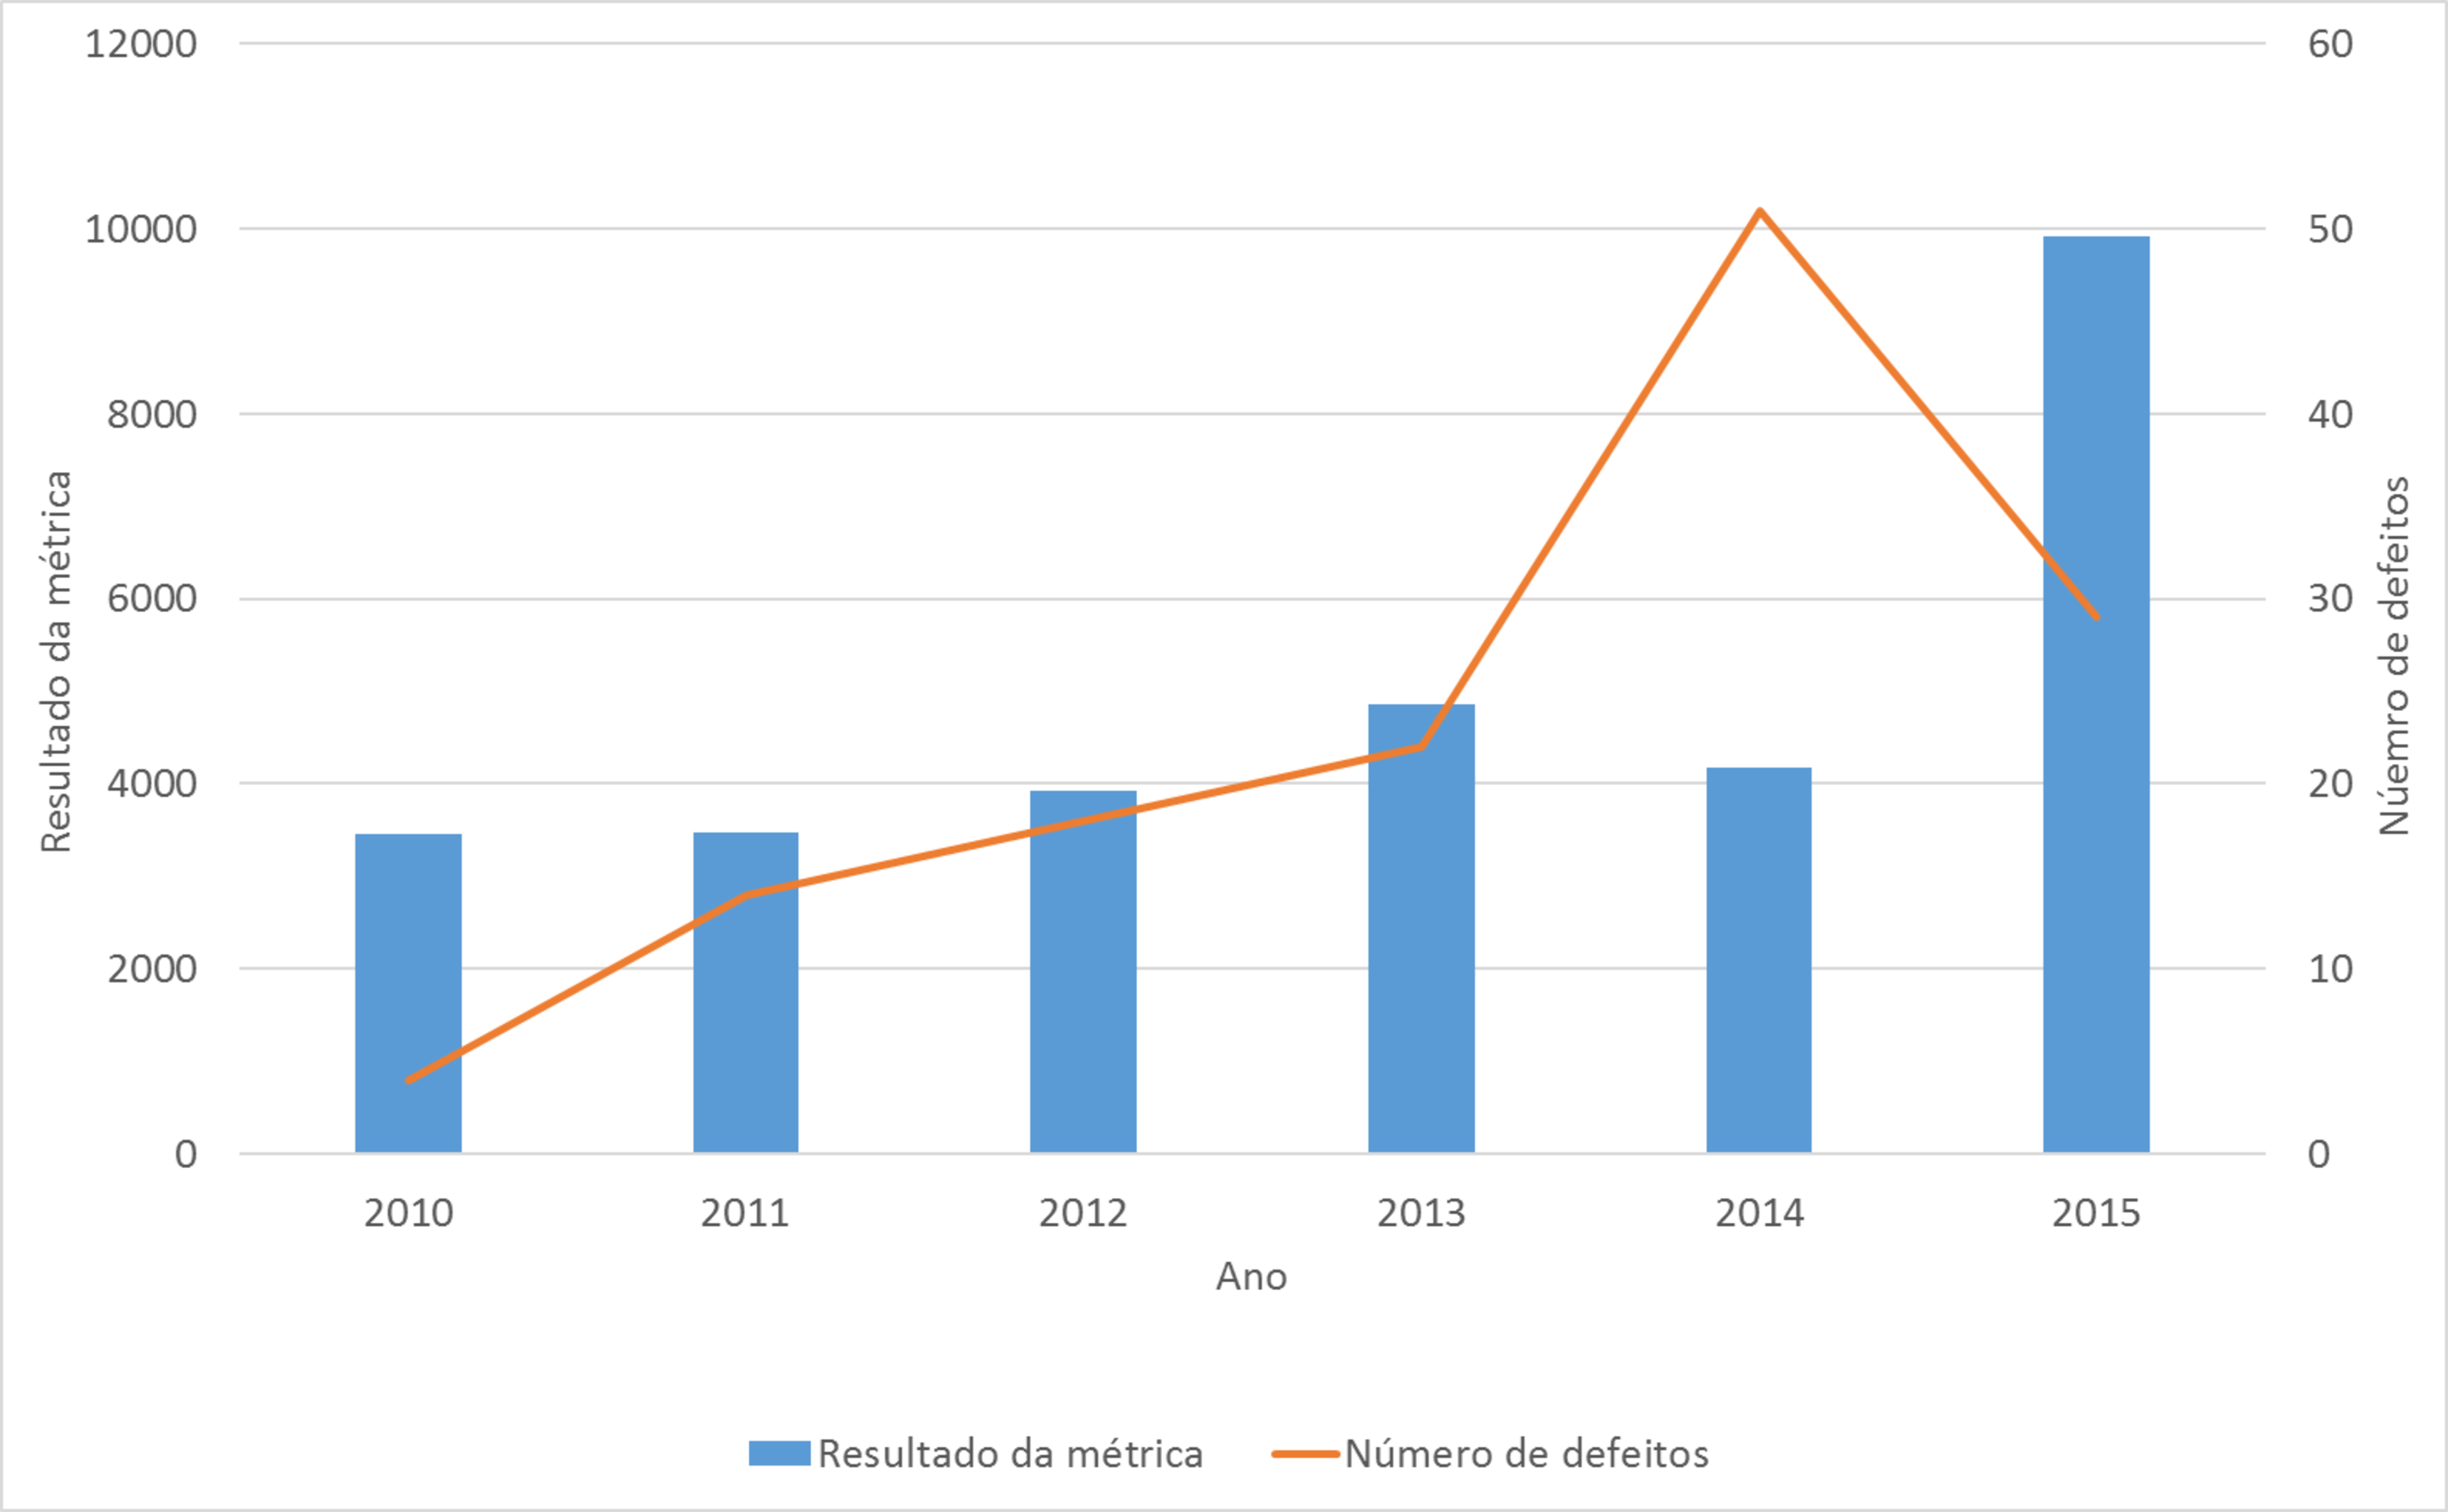
\includegraphics[width=1\textwidth]{./04-figuras/total_issues}
	\fonte{Próprio autor}
	\label{fig:totalXIssue}
\end{figure}

Pode-se notar na \autoref{fig:totalXIssue} que o número de defeitos acompanha a progressão da métrica, mas o pico de cadastro de defeitos não se encontra no mesmo intervalo em que há um pico do resultado da métrica. Este comportamento pode ser explicado pelo fato do \textit{layout} da aplicação ter sofrido uma mudança drástica entre as versões 1.549 e 1.574, disponibilizadas respectivamente em 26/01/2014 e 27/07/2014.

Devido ao valor elevado dos resultados vistos na \autoref{fig:totalXIssue} considerou-se a possibilidade de isolar uma folha de estilo para análise do resultado, partindo do pressuposto que as modificações feitas pela equipe de desenvolvimento são as que impactam e definem a complexidade de manutenção do código. Para tanto foi necessária uma pesquisa no histórico de \textit{commits} dos arquivos CSS do projeto, com intuito de identificar qual arquivo havia sofrido o maior número de alterações ao longo do tempo. Como pode ser visto na \autoref{tab:commits}, o arquivo \texttt{style.css} foi o que sofreu mais \textit{commits}, sendo identificado assim como o arquivo de codificação CSS principal do projeto.

\begin{table}[!htbp]
	\centering
	\caption{Número de commits para cada arquivo CSS renderizado na página princpal do Jenkins.}
	\label{tab:commits}
	\begin{tabular}{l|c}
		\textbf{Arquivo CSS} & \textbf{Número de commits} \\ \hline
		style.css            & 113                        \\
		color.css            & 2                          \\
		responsive-grid.css  & 2                          \\
		yui\textbackslash button.css       & 3                          \\
		yui\textbackslash container.css    & 3                          \\
		yui\textbackslash menu.css         & 3                         
	\end{tabular}
\end{table}

A partir desta identificação, a análise sobre progressão dos resultados e o número de defeitos criados foi refeita considerando somente o arquivo \texttt{style.css} com o intuito de determinar o impacto das modificações feitas na folha de estilo principal do projeto sobre o número de defeitos.

\begin{figure}[!htb]
	\centering
	\caption{Comparação do resultado da métrica do \texttt{style.css} em relação ao número de tarefas criadas.}
	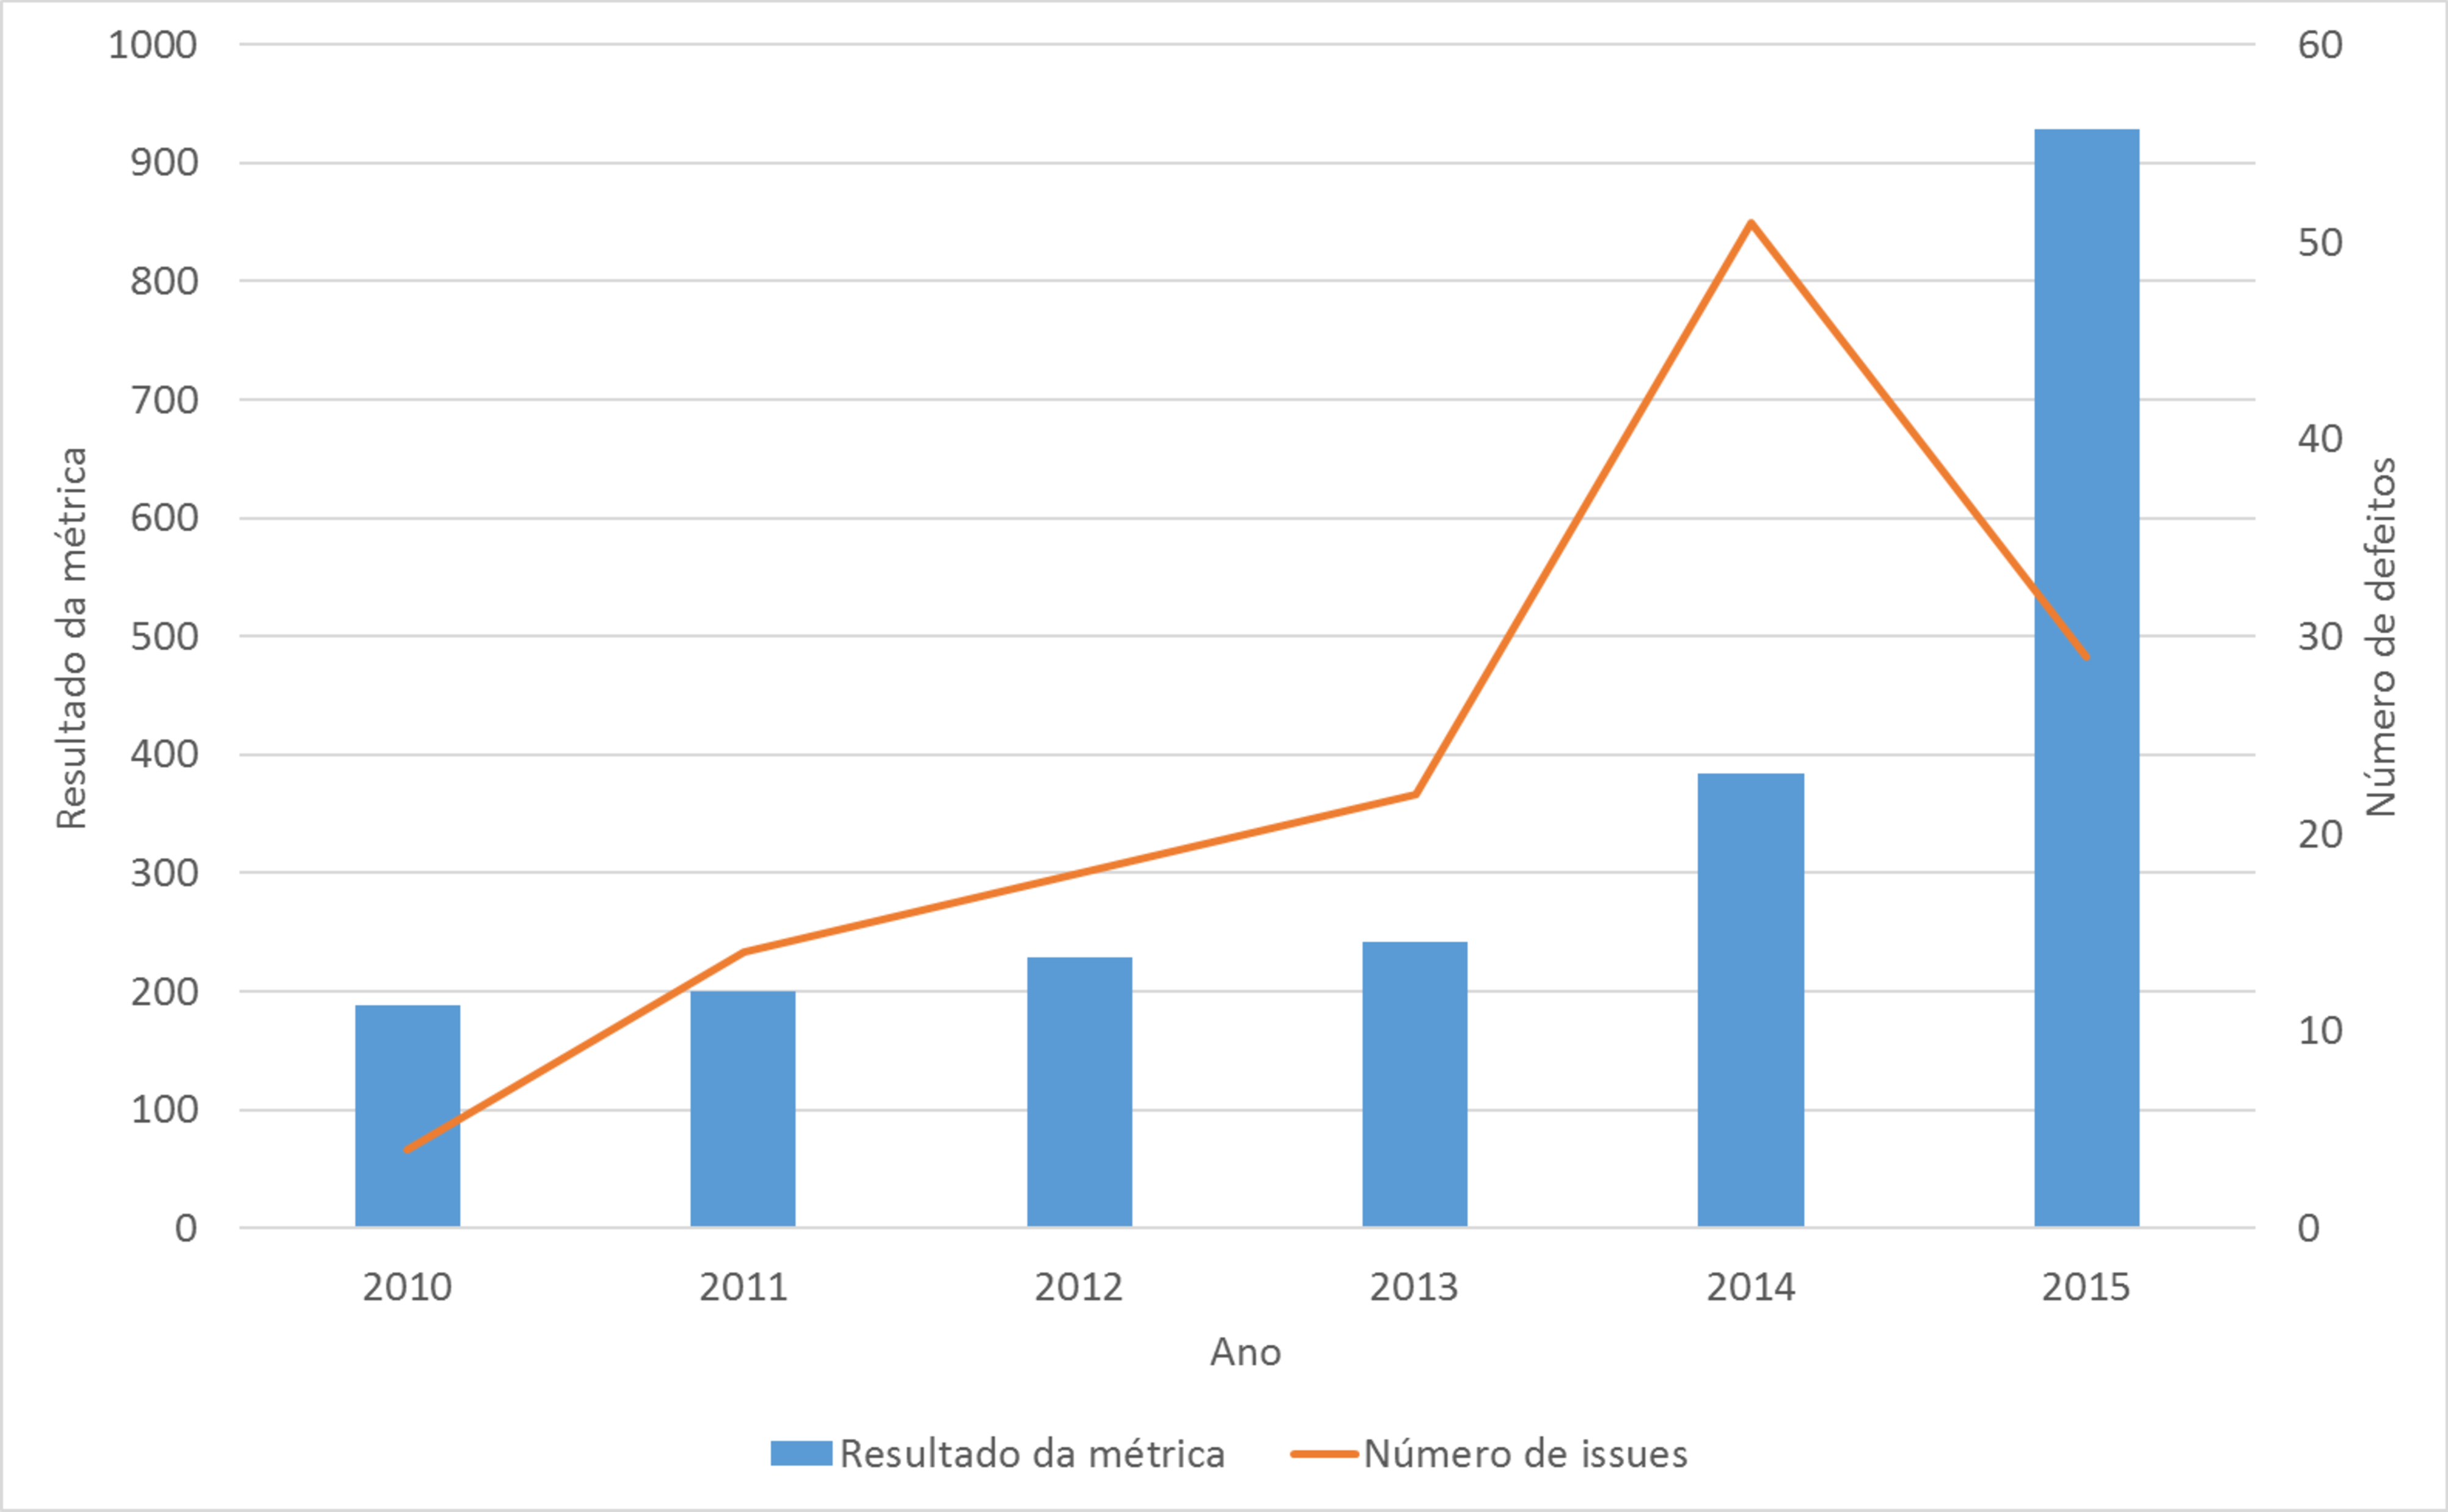
\includegraphics[width=0.9\textwidth]{./04-figuras/style_issues}
	\fonte{Próprio autor}
	\label{fig:styleXIssues}
\end{figure}

Pode-se notar na \autoref{fig:styleXIssues} que a evolução da métrica foi crescente durante toda a progressão temporal e também um aumento considerável do resultado referente à mudança de \textit{layout} em 2014.

O comportamento do resultado da métrica para o arquivo \texttt{style.css} e o agregado é semelhante, o que leva a acreditar que o valor da métrica está relacionado às modificações feitas no projeto. Este comportamento para o arquivo \texttt{style.css} leva a hipótese de que as mudanças na folha de estilo causaram um aumento progressivo no resultado, ou seja, toda nova modificação somou ao valor da métrica.

Esta hipótese põe em questão qual o motivo desta mudança, que deve ser respondida através do estudo da métrica. Sobre quais são os critérios de avaliação que impactam no seu resultado e como esses se comportam. 

\section{Apreciação da métrica}

Com o objetivo de avaliar a contribuição de cada critério no resultado final da métrica, fez-se uma análise da distribuição dentro do total de cada resultado. Na \autoref{fig:compos_crit} pode-se notar uma variação em função do tempo na parcela de contribuição dos critérios. Essa variação pode ser originada a partir da necessidade de se corrigir as regras, ou adicionar novas, para cada uma das situações encontradas durante o período de manutenção.

\begin{figure}[!htb]
	\centering
	\caption{Composição do valor da métrica por cada critério.}
	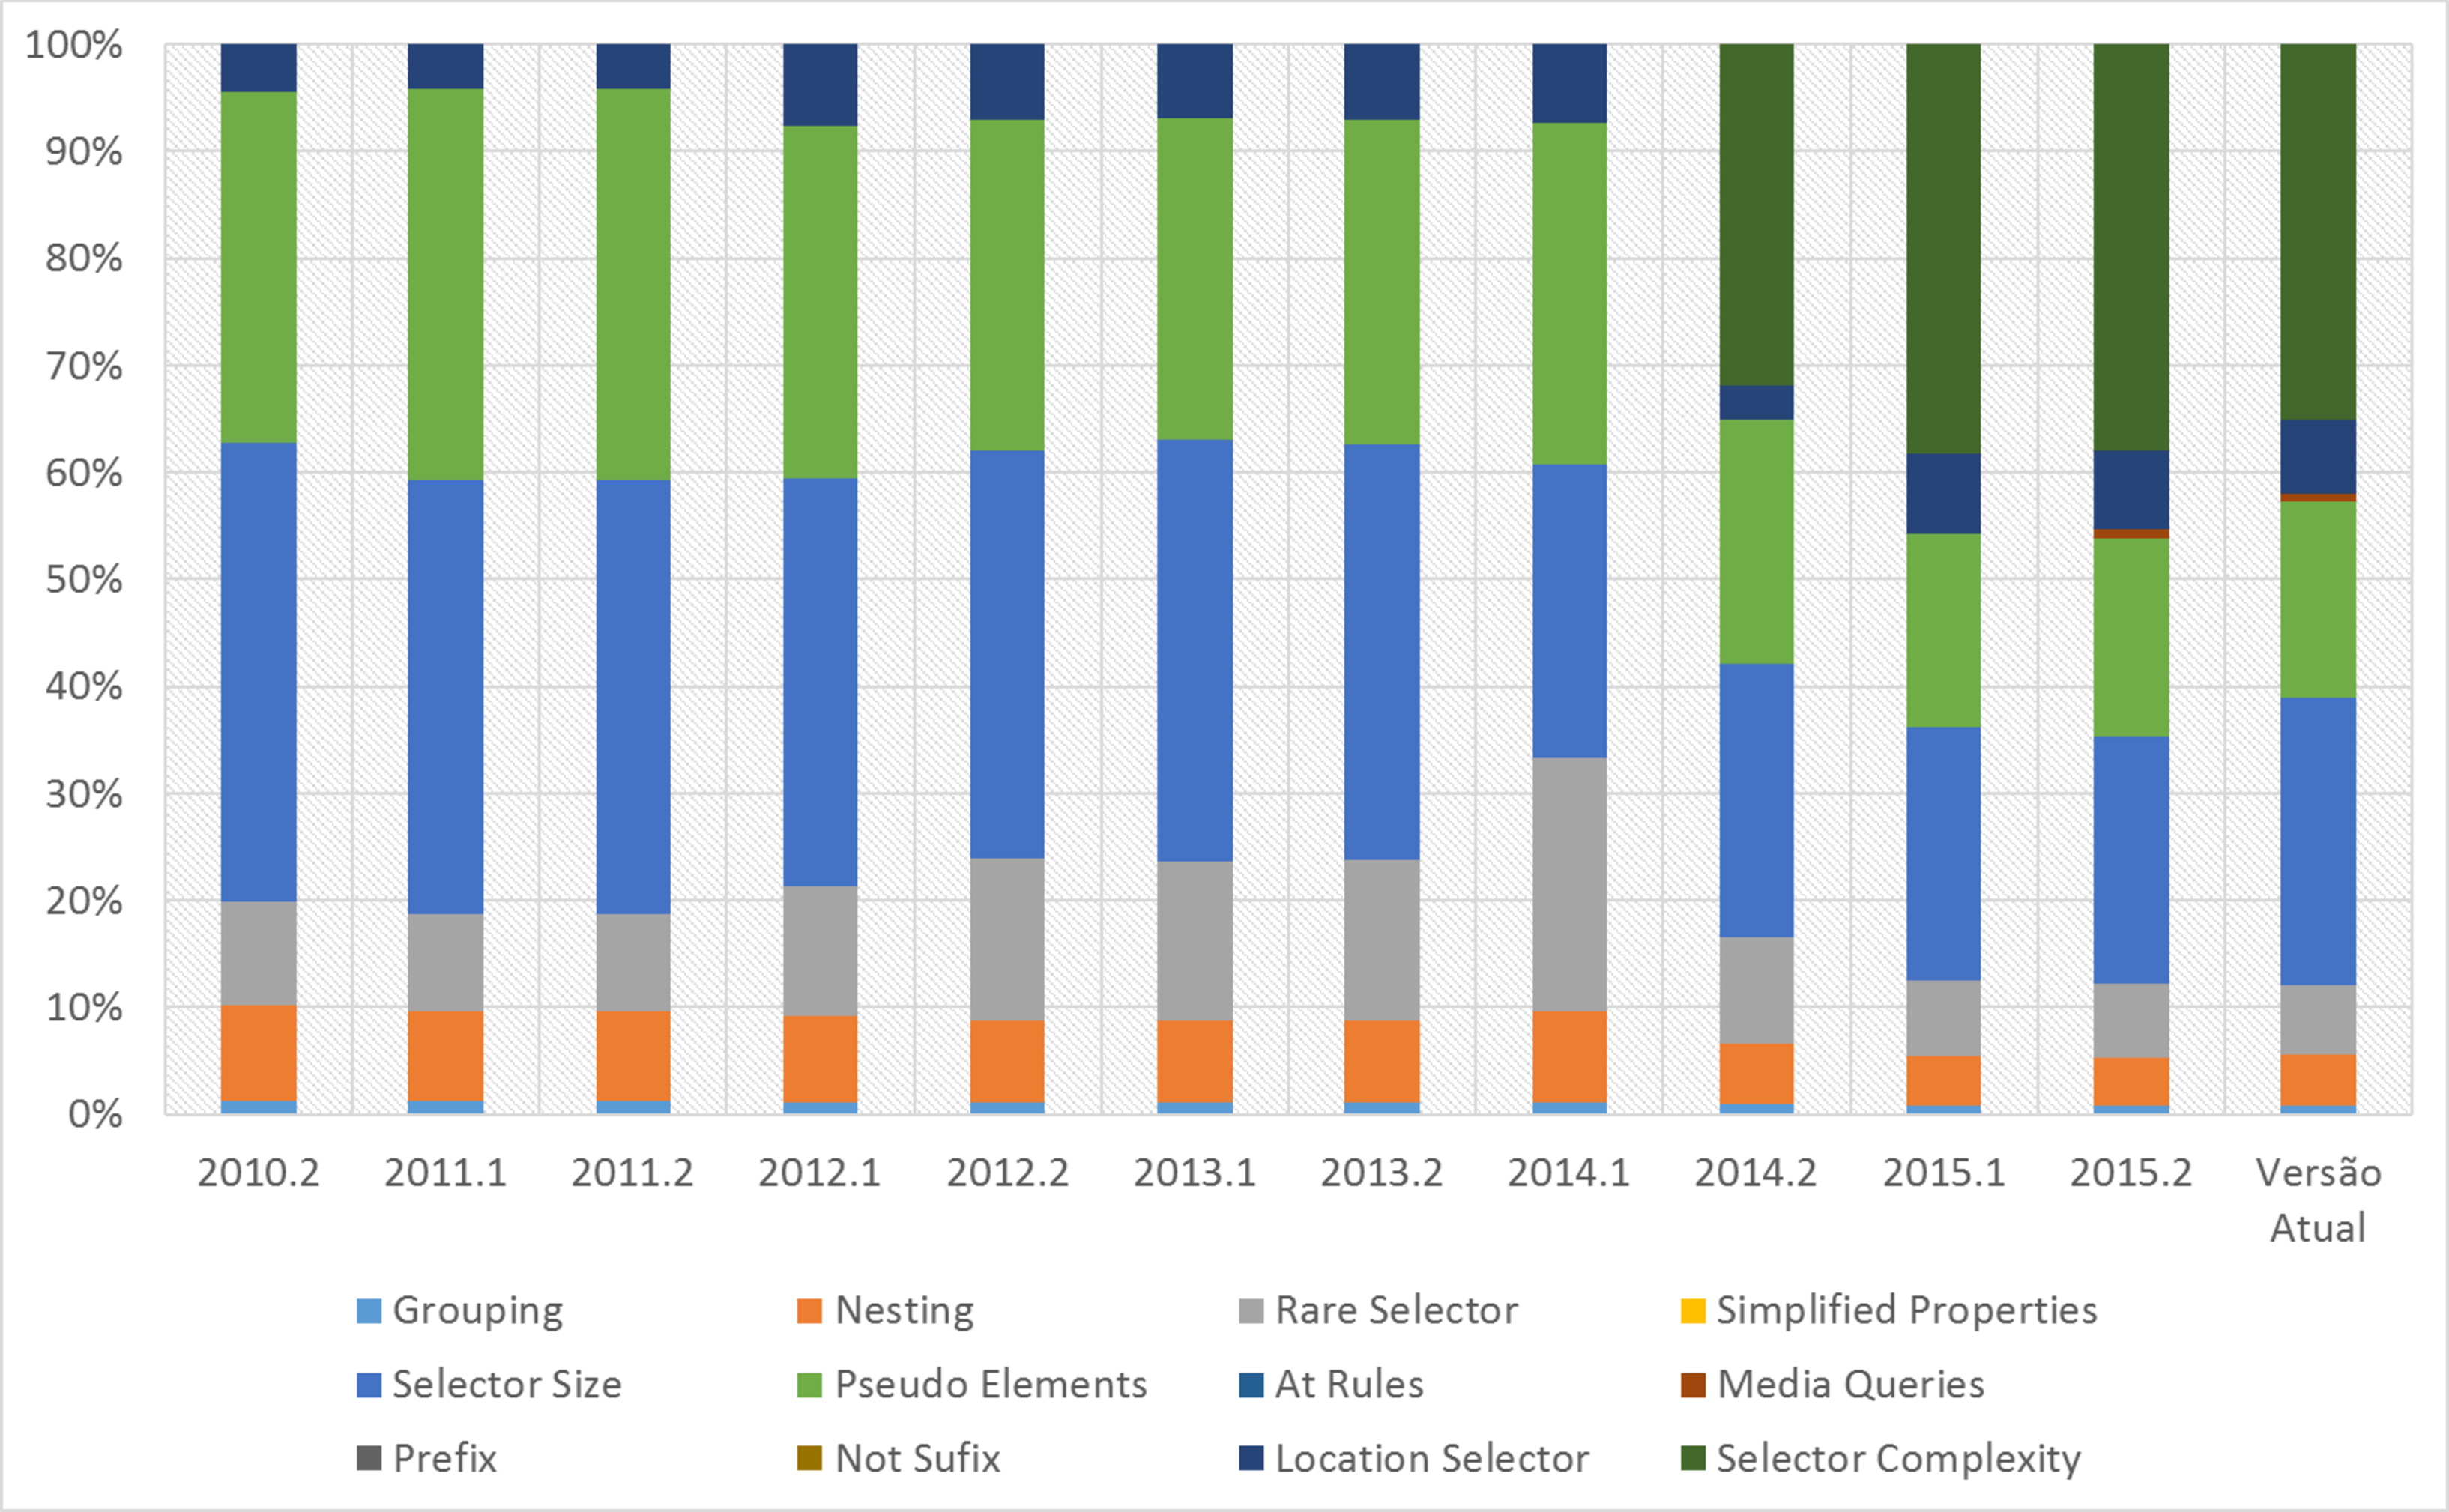
\includegraphics[width=0.9\textwidth]{./04-figuras/composition_criteria}
	\fonte{Próprio autor}
	\label{fig:compos_crit}
\end{figure}

O aumento da contribuição de outros critérios no resultado da métrica, pode ser interpretado como um aumento na complexidade do código.  Através da \autoref{fig:compos_crit}, nota-se que o perfil de complexidade foi se alterando com a evolução do código, o que pode ser explicado pelo aumento da contribuição ou o surgimento de outros critérios que antes não estavam presentes na avaliação da métrica.

Esse aumento de complexidade do código CSS pode ser um agente causador de efeitos colaterais, que por sua vez podem causar um aumento considerável no número de defeitos no estilo de uma página \textit{web}. Esse fato pode explicar o aumento gradativo dos números de defeitos criados acompanhando o resultado da métrica, visto na \autoref{fig:styleXIssues}.

Os resultados obtidos nos testes demonstram um aumento de complexidade do código ao longo do tempo, sendo que essa complexidade impacta no número de defeitos encontrados. Porém, os resultados obtidos não são determinantes, por falta de uma base de comparação. Pode-se concluir então que a métrica apresentada é um passo importante em direção à definição de qualidade de código CSS e pode ser usada como base de comparação para investigações mais profundas de outras aplicações.